\section{Navigation Stack}
\label{section:navigation_stack}

Η πλοήγηση του ρομποτικού οχήματος υλοποιήθηκε με τη χρήση ενός stack πακέτων που προσφέρει το ROS, του navigation\footnote{\href{http://wiki.ros.org/navigation}{http://wiki.ros.org/navigation}}. Αυτό περιέχει ένα σύνολο πακέτων τα οποία χρησιμοποιούν τα δεδομένα της οδομετρίας, των αισθητήρων και του χάρτη του χώρου. Δηλώνοντας ένα σημείο ως στόχο της πλοήγησης δημιουργεί το κατάλληλο σύνολο εντολών ταχύτητας τις οποίες πρέπει να ακολουθήσει το όχημα για να κατευθυνθεί στον στόχο αυτό, χωρίς να συγκρούεται με εμπόδια του περιβάλλοντα χώρου. Η συνολική δομή του stack παρουσιάζεται στο \autoref{fig:navigation_stack_overview}.

\begin{figure}
    \centering
    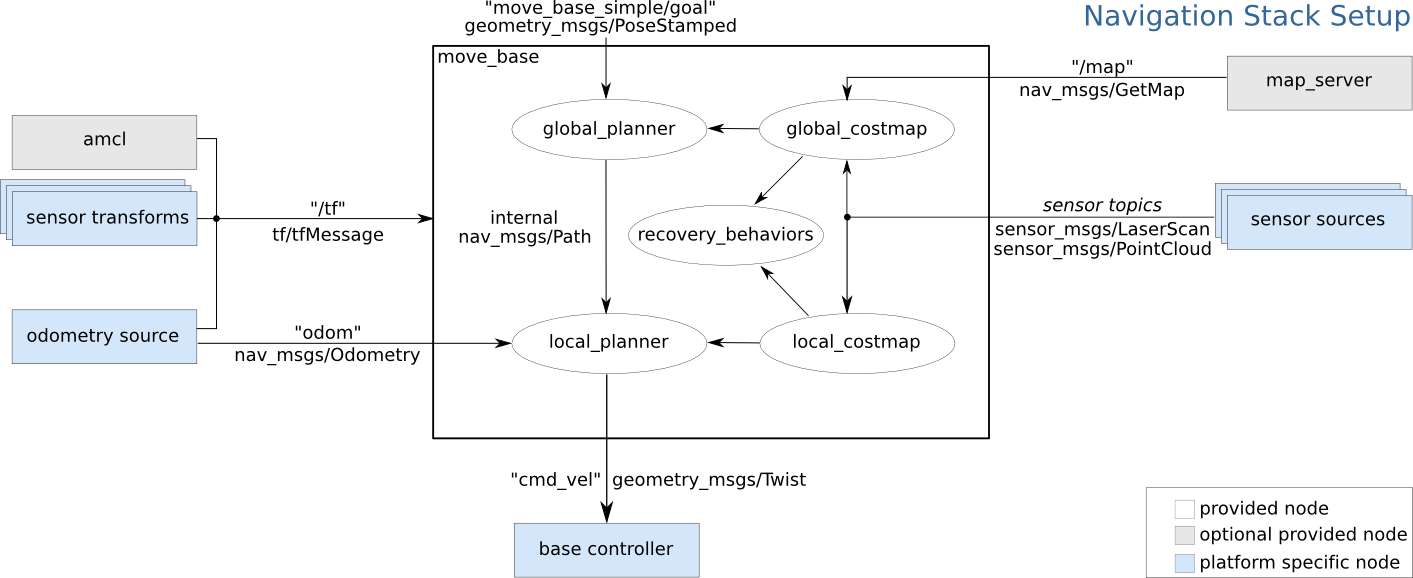
\includegraphics[width=\textwidth]{./images/chapter4/overview_nav_stack.png}
    \caption{Δομή Navigation Stack}
    Πηγή: \href{http://wiki.ros.org/navigation/Tutorials/RobotSetup}{http://wiki.ros.org/navigation/Tutorials/RobotSetup}
    \label{fig:navigation_stack_overview}
\end{figure}

Υπάρχουν, λοιπόν, δύο διαφορετικοί σχεδιαστές μονοπατιών, ο τοπικός (local planner) και ο καθολικός (global planner). Και οι δύο διαβάζουν την τρέχουσα θέση του οχήματος από τη διεργασία amcl και τον χάρτη του χώρου από την διεργασία map\_server και προσπαθούν να δημιουργήσουν μια ασφαλή πορεία μέχρι το σημείο στόχο. Ο global planner δημιουργεί ένα συνολικό μονοπάτι (global path) από την τρέχουσα θέση μέχρι τον στόχο, χωρίς να δίνει ιδιαίτερη έμφαση σε λεπτομερείς κινήσεις και μικρά εμπόδια στο περιβάλλον. Αντίθετα, ο local planner δημιουργεί ένα μονοπάτι με μικρή συνολική απόσταση (local path) που προσπαθεί να προσεγγίσει το global path ελέγχοντας με μεγαλύτερη ακρίβεια για κοντινά εμπόδια και δυναμικές αλλαγές του περιβάλλοντος προσαρμόζοντας τις κινήσεις του οχήματος. Στην εργασία αυτή χρησιμοποιήθηκαν οι εξής:
\begin{itemize}
    \setlength\itemsep{-0.2em}
    \item teb\_local\_planner ,\footnote{\href{http://wiki.ros.org/teb_local_planner}{http://wiki.ros.org/teb_local_planner}}
    \item global\_planner\footnote{\href{http://wiki.ros.org/global_planner}{http://wiki.ros.org/global_planner}}
\end{itemize}

Για την ασφαλή μετάβαση του οχήματος μέσα στον χώρο δημιουργούνται δύο χάρτες με τιμές κόστους (costmaps) που περιέχουν πληροφορίες για τα εμπόδια του χώρου. Ο ένας χάρτης χρησιμοποιείται από τον global planner και χρησιμοποιεί την δομή ολόκληρου του περιβάλλοντος για την δημιουργία του συνολικόυ μονοπατιού πλοήγησης, ενώ ο δεύτερος χρησιμοποιείται από τον local planner για τοπική αποφυγή εμποδίων.






